\documentclass[]{article}
\usepackage{lmodern}
\usepackage{setspace}
\setstretch{2}
\usepackage{amssymb,amsmath}
\usepackage{ifxetex,ifluatex}
\usepackage{fixltx2e} % provides \textsubscript
\ifnum 0\ifxetex 1\fi\ifluatex 1\fi=0 % if pdftex
  \usepackage[T1]{fontenc}
  \usepackage[utf8]{inputenc}
\else % if luatex or xelatex
  \ifxetex
    \usepackage{mathspec}
  \else
    \usepackage{fontspec}
  \fi
  \defaultfontfeatures{Ligatures=TeX,Scale=MatchLowercase}
\fi
% use upquote if available, for straight quotes in verbatim environments
\IfFileExists{upquote.sty}{\usepackage{upquote}}{}
% use microtype if available
\IfFileExists{microtype.sty}{%
\usepackage{microtype}
\UseMicrotypeSet[protrusion]{basicmath} % disable protrusion for tt fonts
}{}
\usepackage[margin=1in]{geometry}
\usepackage{hyperref}
\PassOptionsToPackage{usenames,dvipsnames}{color} % color is loaded by hyperref
\hypersetup{unicode=true,
            pdftitle={Component response rate variation underlies the stability of complex systems},
            pdfauthor={A. Bradley Duthie ( alexander.duthie@stir.ac.uk )},
            colorlinks=true,
            linkcolor=blue,
            citecolor=Blue,
            urlcolor=Blue,
            breaklinks=true}
\urlstyle{same}  % don't use monospace font for urls
\usepackage{graphicx,grffile}
\makeatletter
\def\maxwidth{\ifdim\Gin@nat@width>\linewidth\linewidth\else\Gin@nat@width\fi}
\def\maxheight{\ifdim\Gin@nat@height>\textheight\textheight\else\Gin@nat@height\fi}
\makeatother
% Scale images if necessary, so that they will not overflow the page
% margins by default, and it is still possible to overwrite the defaults
% using explicit options in \includegraphics[width, height, ...]{}
\setkeys{Gin}{width=\maxwidth,height=\maxheight,keepaspectratio}
\IfFileExists{parskip.sty}{%
\usepackage{parskip}
}{% else
\setlength{\parindent}{0pt}
\setlength{\parskip}{6pt plus 2pt minus 1pt}
}
\setlength{\emergencystretch}{3em}  % prevent overfull lines
\providecommand{\tightlist}{%
  \setlength{\itemsep}{0pt}\setlength{\parskip}{0pt}}
\setcounter{secnumdepth}{0}
% Redefines (sub)paragraphs to behave more like sections
\ifx\paragraph\undefined\else
\let\oldparagraph\paragraph
\renewcommand{\paragraph}[1]{\oldparagraph{#1}\mbox{}}
\fi
\ifx\subparagraph\undefined\else
\let\oldsubparagraph\subparagraph
\renewcommand{\subparagraph}[1]{\oldsubparagraph{#1}\mbox{}}
\fi

%%% Use protect on footnotes to avoid problems with footnotes in titles
\let\rmarkdownfootnote\footnote%
\def\footnote{\protect\rmarkdownfootnote}

%%% Change title format to be more compact
\usepackage{titling}

% Create subtitle command for use in maketitle
\newcommand{\subtitle}[1]{
  \posttitle{
    \begin{center}\large#1\end{center}
    }
}

\setlength{\droptitle}{-2em}

  \title{Component response rate variation underlies the stability of complex
systems}
    \pretitle{\vspace{\droptitle}\centering\huge}
  \posttitle{\par}
    \author{A. Bradley Duthie (
\href{mailto:alexander.duthie@stir.ac.uk}{\nolinkurl{alexander.duthie@stir.ac.uk}}
)}
    \preauthor{\centering\large\emph}
  \postauthor{\par}
      \predate{\centering\large\emph}
  \postdate{\par}
    \date{Biological and Environmental Sciences, University of Stirling, Stirling,
UK, FK9 4LA}

\usepackage{amsmath}
\usepackage{natbib}
\usepackage{lineno}
\usepackage[utf8]{inputenc}
\linenumbers
\bibliographystyle{amnatnat}

\begin{document}
\maketitle

\textbf{Key words:} Ecological networks, gene-regulatory networks,
neural networks, financial networks, system stability, random matrix
theory

\subsection{Abstract}\label{abstract}

The stability of a complex system generally decreases with increasing
system size and interconnectivity, a counterintuitive result of
widespread importance across the physical, life, and social sciences.
Despite recent interest in the relationship between system properties
and stability, the effect of variation in the response rate of
individual system components remains unconsidered. Here I vary the
component response rates (\(\boldsymbol{\gamma}\)) of randomly generated
complex systems. I use numerical simulations to show that when component
response rates vary, the potential for system stability is markedly
increased. These results are robust to common network structures,
including small-world and scale-free networks, and cascade food webs.
Variation in \(\boldsymbol{\gamma}\) is especially important for
stability in highly complex systems, in which the probability of
stability would otherwise be negligible. At such extremes of simulated
system complexity, the largest stable complex systems would be unstable
if not for \(\boldsymbol{Var(\gamma)}\). My results therefore reveal a
previously unconsidered aspect of system stability that is likely to be
pervasive across all realistic complex systems.

\subsection{Introduction}\label{introduction}

In 1972, May\textsuperscript{\protect\hyperlink{ref-May1972}{1}} first
demonstrated that randomly assembled systems of sufficient complexity
are almost inevitably unstable given infinitesimally small
perturbations. Complexity in this case is defined by the size of the
system (i.e., the number of potentially interacting components; \(S\)),
its connectance (i.e., the probability that one component will interact
with another; \(C\)), and the variance of interaction strengths
(\(\sigma^{2}\))\textsuperscript{\protect\hyperlink{ref-Allesina2012}{2}}.
May's finding that the probability of local stability falls to near zero
given a sufficiently high threshold of \(\sigma\sqrt{SC}\) is broadly
relevant for understanding the dynamics and persistence of systems such
as
ecological\textsuperscript{\protect\hyperlink{ref-May1972}{1}--\protect\hyperlink{ref-Grilli2017}{5}},
neurological\textsuperscript{\protect\hyperlink{ref-Gray2008}{6},\protect\hyperlink{ref-Gray2009}{7}},
biochemical\textsuperscript{\protect\hyperlink{ref-Rosenfeld2009}{8},\protect\hyperlink{ref-MacArthur2010}{9}},
and
socio-economic\textsuperscript{\protect\hyperlink{ref-May2008}{10}--\protect\hyperlink{ref-Bardoscia2017}{13}}
networks. As such, identifying general principles that affect stability
in complex systems is of wide-ranging importance.

Randomly assembled complex systems can be represented as large square
matrices (\(\mathbf{M}\)) with \(S\) components (e.g., networks of
species\textsuperscript{\protect\hyperlink{ref-Allesina2012}{2}} or
banks\textsuperscript{\protect\hyperlink{ref-Haldane2011}{11}}). One
element of such a matrix, \(M_{ij}\), defines how component \(j\)
affects component \(i\) in the system at a point of
equilibrium\textsuperscript{\protect\hyperlink{ref-Allesina2012}{2}}.
Off-diagonal elements (\(i \neq j\)) therefore define interactions
between components, while diagonal elements (\(i = j\)) define component
self-regulation (\(d\), e.g., carrying capacity in ecological
communities). Traditionally, off-diagonal elements are assigned non-zero
values with a probability \(C\), which are sampled from a distribution
with variance \(\sigma_{M}^{2}\); diagonal elements are set to
\(d = -1\)\textsuperscript{\protect\hyperlink{ref-May1972}{1},\protect\hyperlink{ref-Allesina2012}{2},\protect\hyperlink{ref-Allesina2015}{4}}.
Local system stability is assessed using eigenanalysis, with the system
being stable if the real parts of all eigenvalues (\(\lambda\)) of
\(\mathbf{M}\) are negative
(\(\max\left(\Re(\lambda)\right) < 0\))\textsuperscript{\protect\hyperlink{ref-May1972}{1},\protect\hyperlink{ref-Allesina2012}{2}}.
In a large system (high \(S\)), eigenvalues are distributed
uniformly\textsuperscript{\protect\hyperlink{ref-Tao2010}{14}} within a
circle centred at \(\Re = -1\) (the mean value of diagonal elements) and
\(\Im = 0\), with a radius of
\(\sigma_{M}\sqrt{SC}\)\textsuperscript{\protect\hyperlink{ref-May1972}{1},\protect\hyperlink{ref-Allesina2012}{2},\protect\hyperlink{ref-Allesina2015}{4}}
(Figs 1a and 2a). Local stability of randomly assembled systems
therefore becomes increasingly unlikely as \(S\), \(C\), and
\(\sigma_{M}\) increase.

May's\textsuperscript{\protect\hyperlink{ref-May1972}{1},\protect\hyperlink{ref-Allesina2012}{2}}
stability criterion \(\sigma_{M}\sqrt{SC} < 1\) assumes that the
expected response rates (\(\gamma\)) of individual components to
perturbations of the system are identical, but this is highly unlikely
in any complex system. In ecological communities, for example, the rate
at which population density changes following perturbation will depend
on the generation time of organisms, which might vary by orders of
magnitude among species. Species with short generation times will
respond quickly (high \(\gamma\)) to perturbations relative to species
with long generation times (low \(\gamma\)). Similarly, the speed at
which individual banks respond to perturbations in financial networks,
or individuals or institutions respond to perturbations in complex
social networks, is likely to vary. The effect of such variance on
stability has not been investigated in complex systems theory.
Intuitively, variation in \(\gamma\) (\(\sigma^{2}_{\gamma}\)) might be
expected to decrease system stability by introducing a new source of
variation into the system and thereby increasing \(\sigma_{M}\). Here I
show that, despite higher \(\sigma_{M}\), realistic complex systems
(such that \(S\) is high but finite) are actually more likely to be
stable if their individual component response rates vary. My results are
robust across commonly observed network structures, including
random\textsuperscript{\protect\hyperlink{ref-May1972}{1}},
small-world\textsuperscript{\protect\hyperlink{ref-Watts1998}{15}},
scale-free\textsuperscript{\protect\hyperlink{ref-Albert2002}{16}},
cascade food
web\textsuperscript{\protect\hyperlink{ref-Williams2000}{17}} networks.

\subsection{Results}\label{results}

\textbf{Component response rates of random complex systems}. Complex
systems \(\mathbf{M}\) are built from two matrices, one modelling
component interactions (\(\mathbf{A}\)), and second modelling component
response rates (\(\gamma\)). Both \(\mathbf{A}\) and \(\gamma\) are
square \(S \times S\) matrices. Rows in \(\mathbf{A}\) define how a
given component \(i\) is affected by each component \(j\) in the system,
including itself (where \(i = j\)). Off-diagonal elments of
\(\mathbf{A}\) are independent and identically distributed (i.i.d), and
diagonal elements are set to \(A_{ii} = -1\) as in
May\textsuperscript{\protect\hyperlink{ref-May1972}{1}}. Diagonal
elements of \(\gamma\) are positive, and off-diagonal elements are set
to zero (i.e. \(\gamma\) is a diagonal matrix with positive support).
The distribution of \(\gamma\) over \(S\) components thereby models the
distribution of component response rates. The dynamics of the entire
system \(\mathbf{M}\) can be defined as
follows\textsuperscript{\protect\hyperlink{ref-Patel2018}{18}},

\begin{equation} \label{defM}
M = \gamma A.
\end{equation}

Equation \ref{defM} thereby serves as a null model to investigate how
variation in component response rate (\(\sigma_{\gamma}\)) affects
complex systems. In the absence of such variation
(\(\sigma_{\gamma} = 0\)), \(\gamma\) is set to the identity matrix
(diagonal elements all equal 1) and \(\mathbf{M} = \mathbf{A}\). Under
these conditions, eigenvalues of \(\mathbf{M}\) are distributed
uniformly\textsuperscript{\protect\hyperlink{ref-Tao2010}{14}} in a
circle centred at \((-d, 0)\) with a radius of
\(\sigma_{M} \sqrt{SC}\)\textsuperscript{\protect\hyperlink{ref-May1972}{1}}
(Figure 1a).

\textbf{Effect of \(\mathbf{\sigma^{2}_{\gamma}}\) on \(\mathbf{M}\)
(co)variation}. The value of \(\max(\Re(\lambda))\), and therefore
system stability, can be estimated from five properties of
\(\mathbf{M}\)\textsuperscript{\protect\hyperlink{ref-Tang2014b}{19}}.
These properties include (1) system size (\(S\)), (2) mean
self-regulation of components (\(d\)), (3) mean interaction strength
between components (\(\mu\)), (4) the standard deviation between
component interaction strengths (\(\sigma_{M}\)), and (5) the
correlation of interaction strengths between components, \(M_{ij}\) and
\(M_{ji}\) (\(\rho\)). Positive \(\sigma_{\gamma}\) does not change
\(S\), nor does it necessarily change \(E[d]\) or \(E[\mu]\). What
\(\sigma_{\gamma}\) does change is the total variation in component
interaction strengths (\(\sigma_{M}\)), and \(\rho\). Introducing
variation in \(\gamma\) increases the total variation in the system.
Variation of the off-diagonal elements in \(\mathbf{M}\) is described by
the joint variation of two random variables,

\begin{equation} \label{var_full}
\sigma^{2}_{M} = \sigma^{2}_{A}\sigma^{2}_{\gamma} + \sigma^{2}_{A}E[\gamma_{i}]^{2}+\sigma^{2}_{\gamma}E[A_{ij}]^{2}.
\end{equation}

Given \(E[\gamma_{i}] = 1\) and \(E[A_{ij}] = 0\), equation
\ref{var_full} can be simplified,

\begin{equation} \label{var_reduced}
\sigma^{2}_{M} = \sigma^{2}_{A}(1 + \sigma^{2}_{\gamma}).
\end{equation}

The increase caused by \(\sigma^{2}_\gamma\) can be visualised from the
eigenvalue spectra of \(\textbf{A}\) versus
\(\textbf{M} = \gamma\textbf{A}\) (Figure 1). Given \(d = 0\) and
\(C = 1\), the distribution of eigenvalues of \(\textbf{A}\) and
\(\textbf{M}\) lie within a circle of a radius \(\sigma_{A}\sqrt{S}\)
and \(\sigma_{M}\sqrt{S}\), respectively (Figure 1a vs.~1b). If
\(d \neq 0\), positive \(\sigma^{2}_\gamma\) changes the distribution of
eigenvalues\textsuperscript{\protect\hyperlink{ref-Ahmadian2015}{20}--\protect\hyperlink{ref-Stone2017}{22}},
potentially affecting stability (Figure 1c vs.~1d).

Given \(\sigma^{2}_\gamma = 0\), \(\max(\Re(\lambda))\) decrease
linearly with \(\rho\) such
that\textsuperscript{\protect\hyperlink{ref-Tang2014c}{23}},

\begin{equation} \label{rho_stab}
\max(\Re(\lambda)) \approx \sigma_{M}\sqrt{SC}\left(1 + \rho\right).
\end{equation}

If \(\rho < 0\), such as when \(\textbf{M}\) models a predator-prey
system in which \(M_{ij}\) and \(M_{ji}\) have opposing signs, stability
increases\textsuperscript{\protect\hyperlink{ref-Allesina2012}{2}}. If
diagonal elements of \(\gamma\) vary independently, the magnitude of
\(\rho\) is decreased because \(\sigma^{2}_{\gamma}\) increases the
variance of \(M_{ij}\) without affecting the expected covariance between
\(M_{ij}\) and \(M_{ji}\).

\textbf{Numerical simulations of random \(\mathbf{M}\) with and without
\(\mathbf{\sigma^{2}_{\gamma}}\)}. I used numerical simulations and
eigenanalysis to test how variation in \(\gamma\) affects stability in
random matrices with known properties, comparing the stability of
\(\textbf{A}\) versus \(\mathbf{M} = \gamma\mathbf{A}\). Values of
\(\gamma\) were sampled from a uniform distribution where
\(\gamma_{i} \sim \mathcal{U}(0, 2)\) and \(\sigma^{2}_{\gamma} = 1/3\)
(see Supplementary Information for other distributions, which give
similar results). Diagonal elements of simulated \(\mathbf{A}\) were
standardised to the mean value of sampled \(\gamma\) so that \(E[d]\) of
\(\textbf{M}\) and \(\textbf{M}\) were guaranteed to be identical. Here
I focus on the effect of \(\gamma\) across values of \(\rho\), and for
increasing system sizes (\(S\)) in random and structured networks. By
increasing \(S\), the objective is to determine the effect of \(\gamma\)
as system complexity increases toward the boundary at which stability is
realistic for a finite system.

\textbf{Simulation of random \(\mathbf{M}\) across \(\mathbf{\rho}\)}

Numerical simulations reveal that \(\sigma^{2}_{\gamma} > 0\) results in
a nonlinear relationship between \(\rho\) and \(\max(\Re(\lambda))\),
which can sometimes increase the stability of the system.

\textbf{Simulation of random \(\mathbf{M}\) across \(\mathbf{S}\)}. To
investigate the effect of \(Var(\gamma)\) on stability across systems of
varying complexity, I simulated random \(\mathbf{M}\) matrices at
\(\sigma = 0.4\) and \(C = 1\) across \(S = \{2, 3, ..., 49, 50\}\). One
million \(\mathbf{M}\) were simulated for each \(S\), and the stability
of \(\mathbf{M}\) was assessed given \(\gamma = 1\) versus
\(\gamma \sim \mathcal{U}(0, 2)\). For all \(S > 10\), I found that the
number of stable random systems was higher given \(Var(\gamma)\) than
when \(\gamma = 1\) (Fig. 3; see Supplementary Information for full
table of results), and that the difference between the probabilities of
observing a stable system increased with an increase in \(S\). In other
words, the potential for \(Var(\gamma)\) to affect stability increased
with system complexity and was most relevant for systems on the cusp of
being too complex to be realistically stable. For the highest values of
\(S\), nearly all systems that were stable given \(Var(\gamma)\) would
not have been stable given \(\gamma = 1\).

\textbf{Targeted manipulation of \(\mathbf{\gamma}\)}. To further
investigate the potential of \(Var(\gamma)\) to be stabilising, I used a
genetic algorithm. Genetic algorithms are heuristic tools that mimic
evolution by natural selection, and are useful when the space of
potential solutions (in this case, possible combinations of \(\gamma\)
values leading to stability in a complex system) is too large to search
exhaustively\textsuperscript{\protect\hyperlink{ref-Hamblin2013}{24}}.
Generations of selection on \(\gamma\) value combinations to minimise
\(\max\left(\Re(\lambda)\right)\) demonstrated the potential for
\(Var(\gamma)\) to increase system stability. Across
\(S = \{2, 3, ..., 39, 40\}\), sets of \(\gamma\) values were found that
resulted in stable systems with probabilities that were up to four
orders of magnitude higher than when \(\gamma = 1\) (Fig. 4), meaning
that stability could often be achieved by manipulating \(S\) \(\gamma\)
values rather than \(S \times S\) \(\mathbf{M}\) elements (i.e., by
manipulating component response rates rather than interactions between
components).

\textbf{System feasibility given \(\mathbf{Var(\gamma)}\)} For complex
systems in which individual system components represent the density of
some tangible quantity, it is relevant to consider the feasibility of
the system. Feasibilility assumes that values of all components are
positive at
equilibrium\textsuperscript{\protect\hyperlink{ref-Grilli2017}{5},\protect\hyperlink{ref-Dougoud2018}{25},\protect\hyperlink{ref-Song2018}{26}}.
This is of particular interest for ecological communities because
population density (\(N\)) cannot take negative values, meaning that
ecological systems need to be feasible for stability to be biologically
realistic\textsuperscript{\protect\hyperlink{ref-Dougoud2018}{25}}.
While my results are intended to be general to all complex systems, and
not restricted to species networks, I have also performed a feasibility
analysis on all matrices \(\mathbf{M}\) tested for stability, and
additionally for specific types of ecological
communities\textsuperscript{\protect\hyperlink{ref-Allesina2012}{2}}
(e.g., competitive, mutualist, predator-prey; see Supplementary
Information). I emphasise that \(\gamma\) is not interpreted as
population density in this analysis, but instead as a fundamental
property of species life history such as expected generation time.
Feasibility was unaffected by \(Var(\gamma)\) and instead occurred with
a fixed probability of \(1/2^{S}\), consistent with a recent proof by
Serván et al.\textsuperscript{\protect\hyperlink{ref-Servan2018}{27}}
(see Supplementary Information). Hence, for pure interacting species
networks, variation in component response rate (i.e., species generation
time) does not affect stability at biologically realistic species
densities.

\subsection{Discussion}\label{discussion}

I have shown that the stability of complex systems might often be
contigent upon variation in the response rates of their individual
components, meaning that factors such as rate of trait evolution (in
biological networks), transaction speed (in economic networks), or
communication speed (in social networks) need to be considered when
investigating the stability of complex systems. Variation in component
response rate is more likely to be critical for stability in systems
that are especially complex, and it can ultimately increase the
probability that system stability is observed above that predicted by
May's\textsuperscript{\protect\hyperlink{ref-May1972}{1}} classically
derived \(\sigma \sqrt{SC}\) criterion. The logic outlined here is
general, and potentially applies to any complex system in which
individual system components can vary in their reaction rates to system
perturbation.

It is important to recognise that variation in component response rate
is not stabilising per se; that is, adding variation in component
response rates to a particular system does not increase the probability
that the system will be stable. Rather, highly complex systems that are
observed to be stable are more likely to have varying component response
rates, and for this variation to be critical to their stability (Fig.
3). This is caused by the shift to a non-uniform distribution of
eigenvalues that occurs by introducing \(Var(\gamma)\) (Fig. 1b, 2b),
which can sometimes cause all of the real components of the eigenvalues
of the system matrix to become negative, but might also increase the
real components of eigenvalues.

My focus is distinct from Gibbs et
al.\textsuperscript{\protect\hyperlink{ref-Gibbs2017}{21}}, who applied
the same mathematical framework to investigate how a diagonal matrix
\(\mathbf{X}\) (equivalent to \(\gamma\) in my model) affects the
stability of a community matrix \(\mathbf{M}\) given an interaction
matrix \(\mathbf{A}\) within a generalised Lotka-Volterra model, where
\(\mathbf{M} = \mathbf{XA}\). Gibbs et
al.\textsuperscript{\protect\hyperlink{ref-Gibbs2017}{21}} analytically
demonstrated that the effect of \(\mathbf{X}\) on system stability
decreases exponentially as system size becomes arbitrarily large
(\(S \to \infty\)) for a given magnitude of complexity
\(\sigma\sqrt{SC}\). My numerical results do not contradict this
prediction because I did not scale \(\sigma = 1 / \sqrt{S}\), but
instead fixed \(\sigma\) and increased \(S\) to thereby increase total
system complexity (see Supplemental Information for results simulated
across \(\sigma\) and \(C\)). Overall, I show that component response
rate variation increases the upper bound of complexity at which
stability can be realistically observed, meaning that highly complex
systems are more likely than not to vary in their component response
rates, and for this variation to be critical for system stability.

The potential importance of component response rate variation was most
evident from the results of simulations in which the genetic algorithm
was used in attempt to maximise the probability of system stability. The
probability that some combination of component response rates could be
found to stabilise the system was shown to be up to four orders of
magnitude higher than the background probabilities of stability in the
absence of any component response rate variation. Instead of
manipulating the \(S \times S\) interactions between system components,
it might therefore be possible to manipulate only the \(S\) response
rates of individual system components to achieve stability. Hence,
managing the response rates of system components in a targeted way could
potentially facilitate the stabilisation of complex systems through a
reduction in dimensionality.

Interestingly, while complex systems were more likely to be stable given
variation in component response rate, they were not more likely to be
feasible, meaning that stability was not increased when component values
were also restricted to being positive at equilibrium. Feasibility is
important to consider, particularly for the study of ecological networks
of
species\textsuperscript{\protect\hyperlink{ref-Grilli2017}{5},\protect\hyperlink{ref-Stone2017}{22},\protect\hyperlink{ref-Dougoud2018}{25},\protect\hyperlink{ref-Servan2018}{27}}
because population densities cannot realistically be negative. My
results therefore suggest that variation in the rate of population
responses to perturbation (e.g., due to differences in generation time
among species) is unlikely to be critical to the stability of purely
multi-species interaction networks (see also Supplementary Information).
Nevertheless, ecological interactions do not exist in isolation in
empirical
systems\textsuperscript{\protect\hyperlink{ref-Patel2018}{18}}, but
instead interact with evolutionary, abiotic, or social-economic systems.
The relevance of component response rate for complex system stability
should therefore not be ignored in the broader context of ecological
communities.

A general mathematical framework encompassing shifts in eigenvalue
distributions caused by a vector \(\gamma\) has been
investigated\textsuperscript{\protect\hyperlink{ref-Ahmadian2015}{20}}
and recently applied to questions concerning species density and
feasibility\textsuperscript{\protect\hyperlink{ref-Gibbs2017}{21},\protect\hyperlink{ref-Stone2017}{22}},
but \(\gamma\) has not been interpreted as rates of response of
individual system components to perturbation. My model focuses on
component response rates for systems of a finite size, in which
complexity is high but not yet high enough to make the probability of
stability unrealistically low for actual empirical systems. For this
upper range of system size, randomly assembled complex systems are more
likely to be stable if their component response rates vary (e.g.,
\(10 < S < 30\) for parameter values in Fig. 3). Overall, I suggest that
variation in component response rate might therefore be critical for
maintaining stability in many highly complex empirical systems. These
results are broadly applicable for understanding the stability of
complex networks across the physical, life, and social sciences.

\subsection{Methods}\label{methods}

\textbf{Component response rate variation (\(\mathbf{\gamma}\))}. In a
synthesis of eco-evolutionary feedbacks on community stability, Patel et
al. model a system that includes a vector of potentially changing
species densities (\(\mathbf{N}\)) and a vector of potentially evolving
traits
(\(\mathbf{x}\))\textsuperscript{\protect\hyperlink{ref-Patel2018}{18}}.
For any species \(i\) or trait \(j\), change in species density
(\(N_{i}\)) or trait value (\(x_{j}\)) with time (\(t\)) is a function
of the vectors \(\mathbf{N}\) and \(\mathbf{x}\),

\[\frac{dN_{i}}{dt} = N_{i}f_{i}(\mathbf{N}, \mathbf{x}),\]

\[\frac{dx_{j}}{dt} = \epsilon g_{j}(\mathbf{N}, \mathbf{x}).\]

In the above, \(f_{i}\) and \(g_{j}\) are functions that define the
effects of all species densities and trait values on the density of a
species \(i\) and the value of trait \(j\), respectively. Patel et al.
were interested in stability when the evolution of traits was relatively
slow or fast in comparison with the change in species
densities\textsuperscript{\protect\hyperlink{ref-Patel2018}{18}}, and
this is modulated in the above by the scalar \(\epsilon\). The value of
\(\epsilon\) thereby determines the timescale separation between ecology
and evolution, with high \(\epsilon\) modelling relatively fast
evolution and low \(\epsilon\) modelling relative slow
evolution\textsuperscript{\protect\hyperlink{ref-Patel2018}{18}}.

I use the same principle that Patel et al. use to modulate the relative
rate of evolution to modulate rates of component responses for \(S\)
components. Following
May\textsuperscript{\protect\hyperlink{ref-May1972}{1},\protect\hyperlink{ref-May1973}{28}},
the value of a component \(i\) at time \(t\) (\(v_{i}(t)\)) is affected
by the value of \(j\) (\(v_{j}(t)\)) and \(j\)'s marginal effect on
\(i\) (\(a_{ij}\)), and by \(i\)'s response rate (\(\gamma_{i}\)),

\[\frac{dv_{i}(t)}{dt} = \gamma_{i} \sum_{j=1}^{S}a_{ij}v_{j}(t).\]

In matrix notation\textsuperscript{\protect\hyperlink{ref-May1973}{28}},

\[\frac{d\mathbf{v}(t)}{dt} = \mathbf{\gamma} \mathbf{A}\mathbf{v}(t).\]

In the above, \(\mathbf{\gamma}\) is a diagonal matrix in which elements
correspond to individual component response rates. Therefore,
\(\mathbf{M} = \mathbf{\gamma} \mathbf{A}\) defines the values of system
components and can be analysed using the techniques of
May\textsuperscript{\protect\hyperlink{ref-May1972}{1},\protect\hyperlink{ref-Ahmadian2015}{20},\protect\hyperlink{ref-May1973}{28}}.
In these analyses, row means of \(\mathbf{A}\) are expected to be
identical, but variation around this expectation will naturally arise
due to random sampling of \(\mathbf{A}\) off-diagonal elements and
finite \(S\). In simulations, the total variation in \(\mathbf{M}\) row
means that is attributable to \(\mathbf{A}\) is small relative to that
attributable to \(\mathbf{\gamma}\), especially at high \(S\). Variation
in \(\mathbf{\gamma}\) specifically isolates the effects of differing
component response rates, hence causing differences in expected
\(\mathbf{M}\) row means.

\textbf{Genetic algorithm}. Ideally, to investigate the potential of
\(Var(\gamma)\) for increasing the proportion of stable complex systems,
the search space of all possible \(\gamma\) vectors would be evaluated
for each unique \(\mathbf{M = \gamma A}\). This is technically
impossible because \(\gamma_{i}\) can take any real value between 0-2,
but even rounding \(\gamma_{i}\) to reasonable values would result in a
search space too large to practically explore. Under these conditions,
genetic algorithms are highly useful tools for finding practical
solutions by mimicking the process of biological
evolution\textsuperscript{\protect\hyperlink{ref-Hamblin2013}{24}}. In
this case, the practical solution is finding vectors of
\(\mathbf{\gamma}\) that decrease the most positive real eigenvalue of
\(\mathbf{M}\). The genetic algorithm used achieves this by initialising
a large population of 1000 different potential \(\mathbf{\gamma}\)
vectors and allowing this population to evolve through a process of
mutation, crossover (swaping \(\gamma_{i}\) values between vectors),
selection, and reproduction until either a \(\mathbf{\gamma}\) vector is
found where all \(\Re(\lambda) < 0\) or some ``giving up'' critiera is
met.

For each \(S = \{2, 3, ..., 39, 40\}\), the genetic algorithm was run
for 100000 random \(\mathbf{M}\) (\(\sigma = 0.4\), \(C = 1\)). The
genetic algorithm was initialised with a population of 1000 different
\(\mathbf{\gamma}\) vectors with elements sampled i.i.d from
\(\gamma_{i} \sim \mathcal{U}(0, 2)\). Eigenanalysis was performed on
the \(\mathbf{M}\) resulting from each \(\mathbf{\gamma}\) vector, and
the 20 \(\mathbf{\gamma}\) vectors resulting in \(\mathbf{M}\) with the
lowest \(\max\left(\Re(\lambda)\right)\) each produced 50 clonal
offspring with subsequent random mutation and crossover between the
resulting new generation of 1000 \(\mathbf{\gamma}\) vectors. Mutation
of each \(\gamma_{i}\) in a \(\mathbf{\gamma}\) vector occurred with a
probability of 0.2, resulting in a mutation effect of size
\(\mathcal{N}(0, 0.02)\) being added to generate the newly mutated
\(\gamma_{i}\) (any \(\gamma_{i}\) values that mutated below zero were
multiplied by \(-1\), and any values that mutated above 2 were set to
2). Crossover occurred between two sets of 100 \(\mathbf{\gamma}\)
vectors paired in each generation; vectors were randomly sampled with
replacement among but not within sets. Vector pairs selected for
crossover swapped all elements between and including two \(\gamma_{i}\)
randomly selected with replacement (this allowed for reversal of vector
element positions during crossover; e.g.,
\(\{\gamma_{4}, \gamma_{5}, \gamma_{6}, \gamma_{7}\} \to \{\gamma_{7}, \gamma_{6}, \gamma_{5}, \gamma_{4}\}\)
). The genetic algorithm terminated if a stable \(\mathbf{M}\) was
found, 20 generations occurred, or if the mean \(\mathbf{\gamma}\)
fitness increase between generations was less than 0.01 (where fitness
was defined as \(W_{\gamma} = -\max\left(\Re(\lambda)\right)\) for
\(\mathbf{M}\)).

\textbf{System feasibility}. Dougoud et
al.\textsuperscript{\protect\hyperlink{ref-Dougoud2018}{25}} identify
the following feasibility criteria for ecological systems characterised
by \(S\) interacting species with varying densities in a generalised
Lotka-Volterra model,

\[\mathbf{n^{*}} = -\left(\theta \mathbf{I} + (CS)^{-\delta}\mathbf{J} \right)^{-1}\mathbf{r}.\]

In the above, \(\mathbf{n^{*}}\) is the vector of species densities at
equilibrium. Feasibility is satisfied if all elements in
\(\mathbf{n^{*}}\) are positive. The matrix \(\mathbf{I}\) is the
identity matrix, and the value \(\theta\) is the strength of
intraspecific competition (diagonal elements). Diagonal values are set
to \(-1\), so \(\theta = -1\). The variable \(\delta\) is a
normalisation parameter that modulates the strength of interactions
(\(\sigma\)) for \(\mathbf{J}\). Implicitly, here \(\delta = 0\)
underlying strong interactions. Hence, \((CS)^{-\delta} = 1\), so in the
above, a diagonal matrix of -1s (\(\theta \mathbf{I}\)) is added to
\(\mathbf{J}\), which has a diagonal of all zeros and an off-diagonal
affecting species interactions (i.e., the expression \((CS)^{-\delta}\)
relates to May's\textsuperscript{\protect\hyperlink{ref-May1972}{1}}
stability
criterion\textsuperscript{\protect\hyperlink{ref-Dougoud2018}{25}} by
\(\frac{\sigma}{(CS)^{-\delta}}\sqrt{SC} < 1\), and hence for my
purposes \((CS)^{-\delta} = 1\)). Given
\(\mathbf{A} = \theta\mathbf{I + J}\), the above criteria is therefore
reduced to the below (see
also\textsuperscript{\protect\hyperlink{ref-Servan2018}{27}}),

\[\mathbf{n^{*} = -A^{-1}r}.\]

To check the feasibility criteria for \(\mathbf{M = \gamma A}\), I
therefore evaluated \(\mathbf{-M^{-1}r}\) (\(\mathbf{r}\) elements were
sampled i.i.d. from \(r_{i} \sim \mathcal{N}(0, 0.4^{2})\)). Feasibility
is satisfied if all of the elements of the resulting vector are
positive.

\textbf{Acknowledgements:} I am supported by a Leverhulme Trust Early
Career Fellowship (ECF-2016-376). Conversations with L. Bussière and N.
Bunnefeld, and comments from J. J. Cusack and I. L. Jones, improved the
quality of this work.

\textbf{Supplementary Information:} Full tables of stability results for
simulations across different system size (\(S\)) values, ecological
community types, connectance (\(C\)) values, interaction strengths
(\(\sigma\)), and \(\gamma\) distributions are provided as supplementary
material. An additional table also shows results for how feasibility
changes across \(S\). All code and simulation outputs are publicly
available as part of the RandomMatrixStability package on GitHub
(\url{https://github.com/bradduthie/RandomMatrixStability}).

\textbf{Additional Information:} The author declares no competing
interests. All work was carried out by A. Bradley Duthie, and all code
and data are accessible on
\href{https://github.com/bradduthie/RandomMatrixStability}{GitHub}.

\textbf{References}

\hypertarget{refs}{}
\hypertarget{ref-May1972}{}
1. May, R. M. Will a large complex system be stable? \emph{Nature}
\textbf{238,} 413--414 (1972).

\hypertarget{ref-Allesina2012}{}
2. Allesina, S. \& Tang, S. Stability criteria for complex ecosystems.
\emph{Nature} \textbf{483,} 205--208 (2012).

\hypertarget{ref-Mougi2012}{}
3. Mougi, A. \& Kondoh, M. Diversity of interaction types and ecological
community stability. \emph{Science} \textbf{337,} 349--351 (2012).

\hypertarget{ref-Allesina2015}{}
4. Allesina, S. \emph{et al.} Predicting the stability of large
structured food webs. \emph{Nature Communications} \textbf{6,} 7842
(2015).

\hypertarget{ref-Grilli2017}{}
5. Grilli, J. \emph{et al.} Feasibility and coexistence of large
ecological communities. \emph{Nature Communications} \textbf{8,} (2017).

\hypertarget{ref-Gray2008}{}
6. Gray, R. T. \& Robinson, P. A. Stability and synchronization of
random brain networks with a distribution of connection strengths.
\emph{Neurocomputing} \textbf{71,} 1373--1387 (2008).

\hypertarget{ref-Gray2009}{}
7. Gray, R. T. \& Robinson, P. A. Stability of random brain networks
with excitatory and inhibitory connections. \emph{Neurocomputing}
\textbf{72,} 1849--1858 (2009).

\hypertarget{ref-Rosenfeld2009}{}
8. Rosenfeld, S. Patterns of stochastic behavior in dynamically unstable
high-dimensional biochemical networks. \emph{Gene Regulation and Systems
Biology} \textbf{3,} 1--10 (2009).

\hypertarget{ref-MacArthur2010}{}
9. MacArthur, B. D., Sanchez-Garcia, R. J. \& Ma'ayan, A. Microdynamics
and criticality of adaptive regulatory networks. \emph{Physics Review
Letters} \textbf{104,} 168701 (2010).

\hypertarget{ref-May2008}{}
10. May, R. M., Levin, S. A. \& Sugihara, G. Complex systems: Ecology
for bankers. \emph{Nature} \textbf{451,} 893--895 (2008).

\hypertarget{ref-Haldane2011}{}
11. Haldane, A. G. \& May, R. M. Systemic risk in banking ecosystems.
\emph{Nature} \textbf{469,} 351--355 (2011).

\hypertarget{ref-Suweis2014}{}
12. Suweis, S. \& D'Odorico, P. Early warning signs in social-ecological
networks. \emph{PLoS ONE} \textbf{9,} (2014).

\hypertarget{ref-Bardoscia2017}{}
13. Bardoscia, M., Battiston, S., Caccioli, F. \& Caldarelli, G.
Pathways towards instability in financial networks. \emph{Nature
Communications} \textbf{8,} 1--7 (2017).

\hypertarget{ref-Tao2010}{}
14. Tao, T. \& Vu, V. Random matrices: Universality of ESDs and the
circular law. \emph{Annals of Probability} \textbf{38,} 2023--2065
(2010).

\hypertarget{ref-Watts1998}{}
15. Watts, D. J. \& Strogatz, S. H. Collective dynamics of 'small world'
networks. \emph{Nature} \textbf{393,} 440--442 (1998).

\hypertarget{ref-Albert2002}{}
16. Albert, R. \& Barabási, A. L. Statistical mechanics of complex
networks. \emph{Reviews of Modern Physics} \textbf{74,} 47--97 (2002).

\hypertarget{ref-Williams2000}{}
17. Williams, R. J. \& Martinez, N. D. Simple rules yield complex food
webs. \emph{Nature} \textbf{404,} 180--183 (2000).

\hypertarget{ref-Patel2018}{}
18. Patel, S., Cortez, M. H. \& Schreiber, S. J. Partitioning the
effects of eco-evolutionary feedbacks on community stability.
\emph{American Naturalist} \textbf{191,} 1--29 (2018).

\hypertarget{ref-Tang2014b}{}
19. Tang, S. \& Allesina, S. Reactivity and stability of large
ecosystems. \emph{Frontiers in Ecology and Evolution} \textbf{2,} 1--8
(2014).

\hypertarget{ref-Ahmadian2015}{}
20. Ahmadian, Y., Fumarola, F. \& Miller, K. D. Properties of networks
with partially structured and partially random connectivity.
\emph{Physical Review E - Statistical, Nonlinear, and Soft Matter
Physics} \textbf{91,} 012820 (2015).

\hypertarget{ref-Gibbs2017}{}
21. Gibbs, T., Grilli, J., Rogers, T. \& Allesina, S. The effect of
population abundances on the stability of large random ecosystems.
\emph{Physical Review E - Statistical, Nonlinear, and Soft Matter
Physics} \textbf{98,} 022410 (2018).

\hypertarget{ref-Stone2017}{}
22. Stone, L. The feasibility and stability of large complex biological
networks: a random matrix approach. \emph{Scientific Reports}
\textbf{8,} 8246 (2018).

\hypertarget{ref-Tang2014c}{}
23. Tang, S., Pawar, S. \& Allesina, S. Correlation between interaction
strengths drives stability in large ecological networks. \textbf{17,}
1094--1100 (2014).

\hypertarget{ref-Hamblin2013}{}
24. Hamblin, S. On the practical usage of genetic algorithms in ecology
and evolution. \emph{Methods in Ecology and Evolution} \textbf{4,}
184--194 (2013).

\hypertarget{ref-Dougoud2018}{}
25. Dougoud, M., Vinckenbosch, L., Rohr, R., Bersier, L.-F. \& Mazza, C.
The feasibility of equilibria in large ecosystems: a primary but
neglected concept in the complexity-stability debate. \emph{PLOS
Computational Biology} \textbf{14,} e1005988 (2018).

\hypertarget{ref-Song2018}{}
26. Song, C. \& Saavedra, S. Will a small randomly assembled community
be feasible and stable? \emph{Ecology} \textbf{99,} 743--751 (2018).

\hypertarget{ref-Servan2018}{}
27. Serván, C. A., Capitán, J. A., Grilli, J., Morrison, K. E. \&
Allesina, S. Coexistence of many species in random ecosystems.
\emph{Nature Ecology and Evolution} \textbf{2,} 1237--1242 (2018).

\hypertarget{ref-May1973}{}
28. May, R. M. Qualitative stability in model ecosystems. \emph{Ecology}
\textbf{54,} 638--641 (1973).

\clearpage

\textbf{Figure 1: Eigenvalue distributions of random complex systems.}
Each panel shows the real (x-axis) and imaginary (y-axis) parts of
\(S =\) 400 eigenvalues from random \(S \times S\) matrices.
(\(\textbf{a}\)) A system represented by a matrix \(\mathbf{A}\), in
which all elements are sampled from a normal distribution with
\(\mu = 0\) and \(\sigma_{A} = 1/\sqrt{S}\). Points are uniformly
distributed within a circle centred at the origin with a radius of
\(\sigma_{A} \sqrt{S} = 1\). (\(\textbf{b}\)) The same system after
including variation in the response rates of \(S\) components,
represented by the diagonal matrix \(\gamma\), such that
\(\mathbf{M} = \gamma\mathbf{A}\). Elements of \(\gamma\) are randomly
sampled from a uniform distribution from \(\min = 0\) to \(\max = 2\).
Eigenvalues of \(\mathbf{M}\) are then distributed non-uniformly within
a circle centred at the origin with a radius of
\(\sqrt{\sigma^{2}_{A}(1 + \sigma^{2}_{\gamma})S} \approx\) 1.14.
(\(\textbf{c}\)) A different random system \(\mathbf{A}\) constructed
from the same parameters as in \(\textbf{a}\), except with diagonal
values of \(-1\). (\(\textbf{d}\)) The same system \(\textbf{c}\) after
including variation in component response rates, sampled from
\(\mathcal{U}(0, 2)\) as in \(\textbf{b}\).

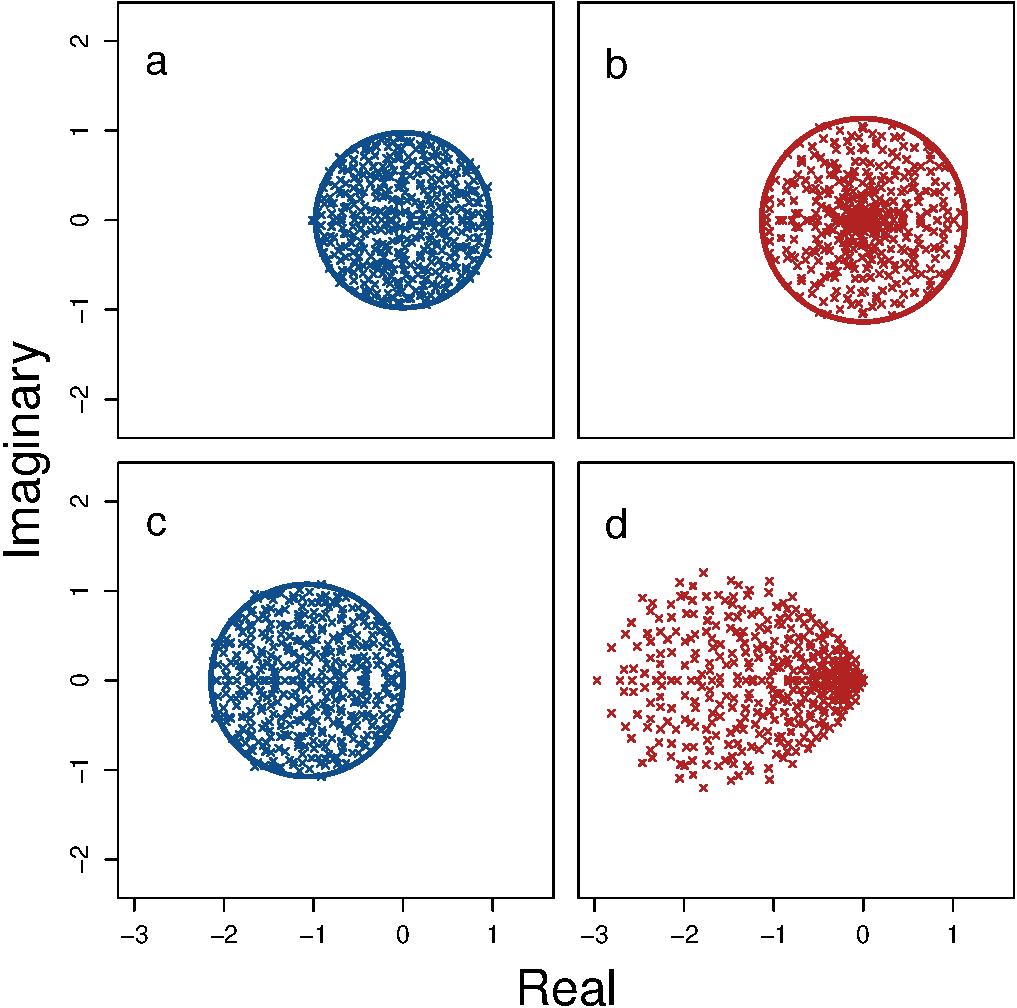
\includegraphics{ms_files/figure-latex/unnamed-chunk-9-1.pdf}

\clearpage

\textbf{Figure 2: Complex system correlation versus stability with and
without variation in component response rates}. Each point represents
10000 replicate numerical simulations of a random complex system
\(\mathbf{M} = \gamma \mathbf{A}\) with a fixed correlation between
off-diagonal elements \(A_{ij}\) and \(A_{ji}\) (\(\rho\), x-axis).
Where real parts of eigenvalues of \(\mathbf{M}\) are negative (y-axis),
\(\mathbf{M}\) is stable (black dotted line). Blue circles show systems
in the absence of variation in component response rates
(\(\sigma^{2}_{\gamma} = 0\)). Red squares show systems in which
\(\sigma^{2}_{\gamma} = 1/3\). Arrows show the range of real parts of
leading eigenvalues observed. Because \(\gamma\) decreases the magnitude
of \(\rho\), purple lines are included to link replicate simulations
before (blue circles) and after (red squares) including \(\gamma\). The
range of \(\rho\) values in which \(\gamma\) decreases the mean real
part of the leading eigenvalue is indicated with grey shading. In all
simulations, system size and connectence were set to \(S = 25\) and
\(C = 1\), respectively. Off-diagonal elements of \(\textbf{A}\) were
randomly sampled from \(A_{ij} \sim \mathcal{N}(0, 0.4)\), and diagonal
elements were set to \(-1\). Elements of \(\gamma\) were sampled,
\(\gamma_{i} \sim \mathcal{U}(0, 2)\).

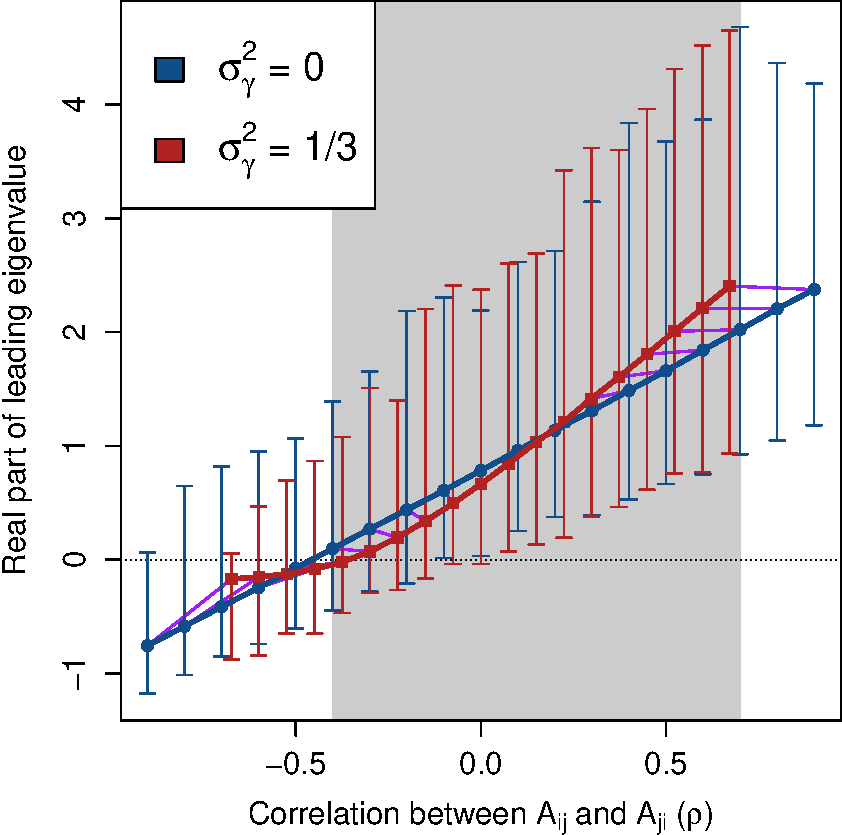
\includegraphics{ms_files/figure-latex/unnamed-chunk-12-1.pdf}

\clearpage

\textbf{Figure 3: System correlation versus stability across different
system sizes}. In each panel, 10000 random complex systems
\(\mathbf{M} = \gamma \mathbf{A}\) are simulated for each correlation
\(\rho = \{-0.90, -0.85, ..., 0.85, 0.90 \}\) between off-diagonal
elements \(A_{ij}\) and \(A_{ji}\). Lines show the expected real part of
the leading eigenvalues of \(\mathbf{M}\) (red squares) versus
\(\mathbf{A}\) (blue circles) across \(\rho\), where negative values
(below the dotted black line) indicate system stability. Differences
between lines thereby show the effect of component response rate
variation (\(\gamma\)) on system stability across system correlations
and sizes (\(S\)). For all simulations, system connectance was
\(C = 1\). Off-diagonal elements of \(\textbf{A}\) were randomly sampled
from \(A_{ij} \sim \mathcal{N}(0, 0.2)\), and diagonal elements were set
to \(-1\). Elements of \(\gamma\) were sampled such that
\(\gamma_{i} \sim \mathcal{U}(0, 2)\), so \(\sigma^{2}_{\gamma} = 1/3\).

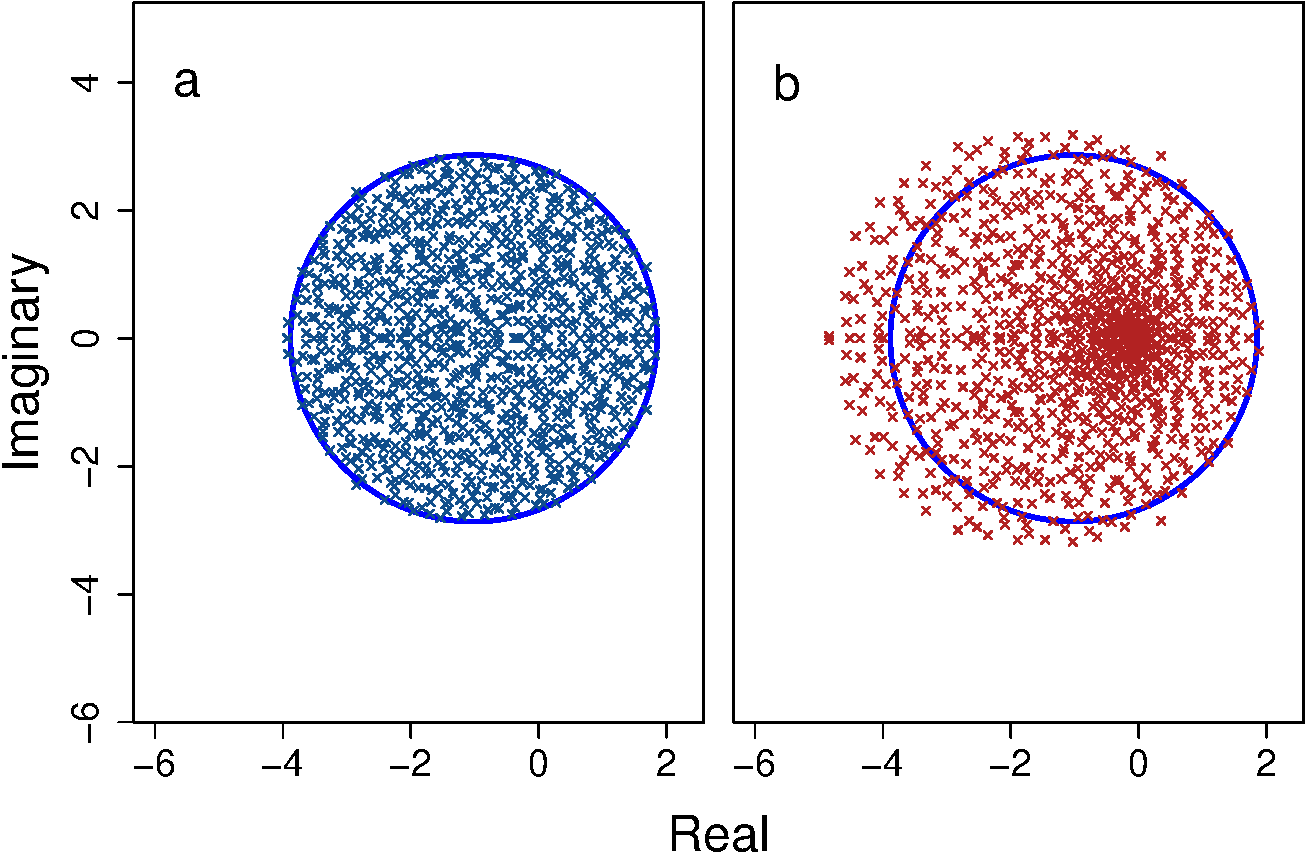
\includegraphics{ms_files/figure-latex/unnamed-chunk-13-1.pdf}

\clearpage

\textbf{Figure 4: Stability of large complex systems with and without
variation in component response rate (\(\boldsymbol{\gamma}\)).} The
\(\ln\) number of systems that are stable across different system sizes
(\(S = \{2, 3, ..., 49, 50 \}\)) given \(C = 1\), and the proportion of
systems in which variation in \(\gamma\) is critical for system
stability. For each \(S\), 1 million complex systems are randomly
generated. Stability of each complex system is tested given variation in
\(\gamma\) by randomly sampling \(\gamma \sim \mathcal{U}(0, 2)\).
Stability given \(\sigma^{2}_{\gamma}>0\) is then compared to stability
in an otherwise identical system in which
\(\gamma = E[\mathcal{U}(0, 2)]\) for all components. Blue and red bars
show the number of stable systems in the absence and presence of
\(\sigma^{2}_{\gamma}\), respectively. The black line shows the
proportion of systems that are stable when \(\sigma^{2}_{\gamma}>0\),
but would be unstable if \(\sigma^{2}_{\gamma}=0\).

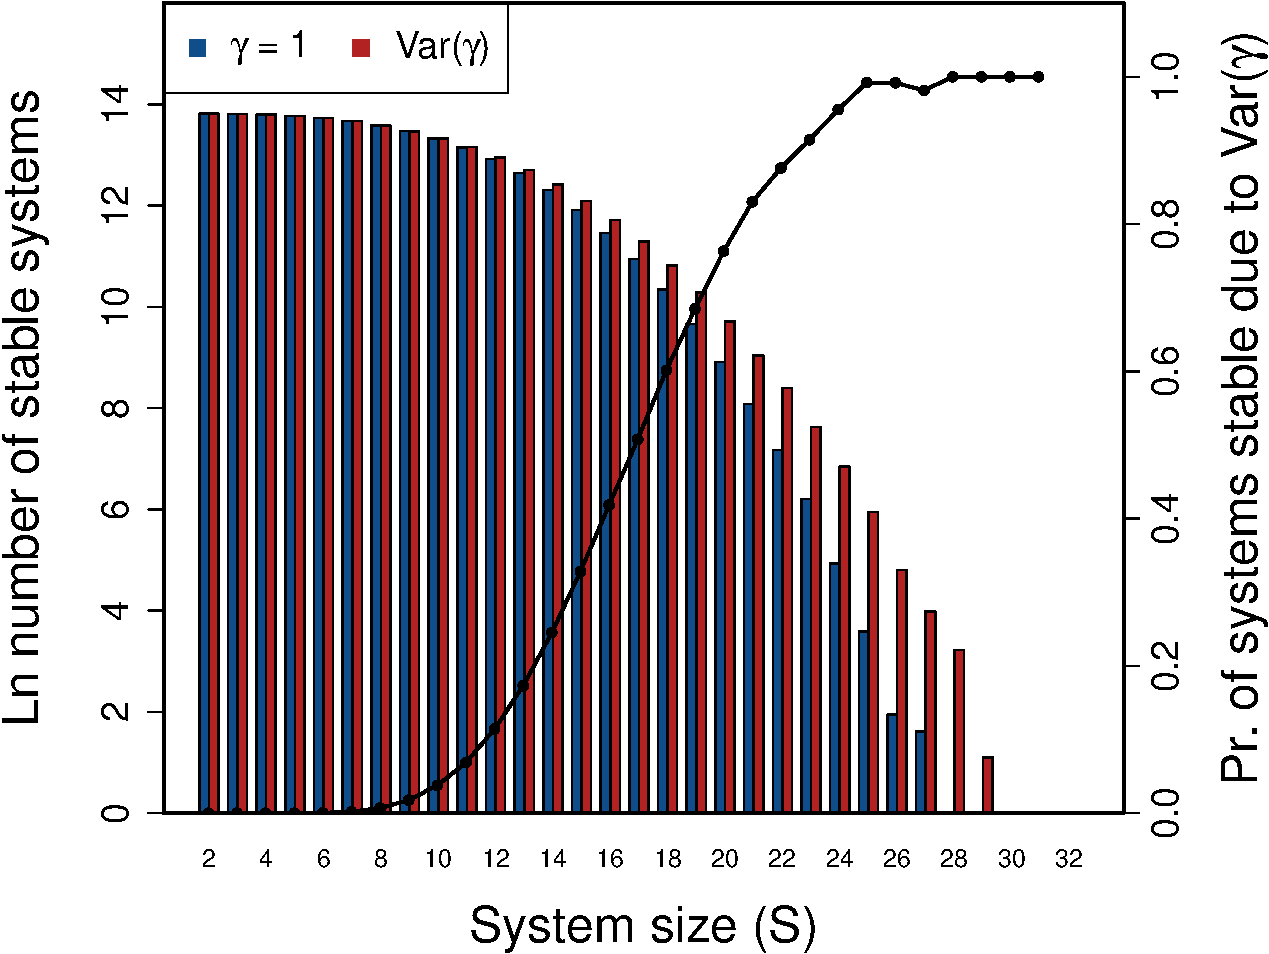
\includegraphics{ms_files/figure-latex/unnamed-chunk-15-1.pdf}


\end{document}
